% NOTES
% https://www.elsevier.com/journals/journal-of-cleaner-production/0959-6526/guide-for-authors
% Original article: Standard research papers of 6000-8000 words in length, with tables, illustrations and references, in which hypotheses are tested and results reported.
% Limit 20000 Characters	

% We might have to or should add a Data in Brief: https://www.elsevier.com/journals/data-in-brief/2352-3409/guide-for-authors

% Math formulae
% Please submit math equations as editable text and not as images. Present simple formulae in line with normal text where possible and use the solidus (/) instead of a horizontal line for small fractional terms, e.g., X/Y. In principle, variables are to be presented in italics. Powers of e are often more conveniently denoted by exp. Number consecutively any equations that have to be displayed separately from the text (if referred to explicitly in the text).

\documentclass[review]{elsarticle}

\usepackage{epstopdf}
\usepackage{lineno,hyperref}
\usepackage{booktabs}
\usepackage{float}
\usepackage{amsmath}
\usepackage{siunitx}
\usepackage{textcomp}
\modulolinenumbers[5]

\renewcommand*{\sectionautorefname}{Section}
\renewcommand*{\figureautorefname}{Figure}
\renewcommand*{\tableautorefname}{Table}
\renewcommand*{\equationautorefname}{Eq.}

\journal{Journal of Cleaner Production}

%%%%%%%%%%%%%%%%%%%%%%%
%% Elsevier bibliography styles
%%%%%%%%%%%%%%%%%%%%%%%
%% To change the style, put a % in front of the second line of the current style and
%% remove the % from the second line of the style you would like to use.
%%%%%%%%%%%%%%%%%%%%%%%

%% Numbered
%\bibliographystyle{model1-num-names}

%% Numbered without titles
%\bibliographystyle{model1a-num-names}

%% Harvard
%\bibliographystyle{model2-names.bst}\biboptions{authoryear}

%% Vancouver numbered
%\usepackage{numcompress}\bibliographystyle{model3-num-names}

%% Vancouver name/year
%\usepackage{numcompress}\bibliographystyle{model4-names}\biboptions{authoryear}

%% APA style
%\bibliographystyle{model5-names}\biboptions{authoryear}

%% AMA style
%\usepackage{numcompress}\bibliographystyle{model6-num-names}

%% `Elsevier LaTeX' style
\bibliographystyle{elsarticle-num}
%%%%%%%%%%%%%%%%%%%%%%%

\begin{document}

%%%%%%%%%%%%%%%%%%%%%%%%%%%%%%%%%%%%%%%%%%%%%%%%%%%%%%%%%%%%%%%%%%%%%%%%%%%%%%%%%%%%%
\begin{frontmatter}

\title{Fuel switch, savings, electrification - Decarbonisation in industry OR Pathways to Carbon Neutral Industrial Sectors: Integrated Modelling Approach with High Level of Detail for End-use Processes OR Decarbonization options in industry and conceptual model of industry in the integrated energy system}

%% Group authors per affiliation:

\author[mymainaddress]{Frauke Wiese\corref{mycorrespondingauthor}}
\cortext[mycorrespondingauthor]{Corresponding author}
\ead{frwi@dtu.dk}

\author[mymainaddress]{Mattia Baldini}

\address[mymainaddress]{DTU Management Engineering, Technical University of Denmark}

%%%%%%%%%%%%%%%%%%%%%%%%%%%%%%%%%%%%%%%%%%%%%%%%%%%%%%%%%%%%%%%%%%%%%%%%%%%%%%%%%%%%%
\begin{abstract}
% A concise and factual abstract is required. The abstract should state briefly the purpose of the research, the principal results and major conclusions. An abstract is often presented separately from the article, so it must be able to stand alone. For this reason, References should be avoided, but if essential, then cite the author(s) and year(s). Also, non-standard or uncommon abbreviations should be avoided, but if essential they must be defined at their first mention in the abstract itself.



Main question:
\begin{itemize}
    \item \textbf{Should be rather present a conceptual model how to integrate industry in an integrated energy system model OR} 
    \item should we rather do some calculations without the model based on the numbers we have and describe these?
    \item Maybe we can combine it by backing up the model (deriving the model from ) the data and structure of data we prepared for Denmark, then a result can be the features the model needs to have and the main rough numbers which need to be checked by a model having the features of the conceptual model.
    \item What is the fuel switch options to which cost: Maybe we should have a table with the sectors and end-uses their options to decarbonize. This we can already derive without the model runs
\end{itemize}

\end{abstract}
%%%%%%%%%%%%%%%%%%%%%%%%%%%%%%%%%%%%%%%%%%%%%%%%%%%%%%%%%%%%%%%%%%%%%%%%%%%%%%%%%%%%%

\begin{keyword}
% Immediately after the abstract, provide a maximum of 6 keywords, using American spelling and avoiding general and plural terms and multiple concepts (avoid, for example, 'and', 'of'). Be sparing with abbreviations: only abbreviations firmly established in the field may be eligible. These keywords will be used for indexing purposes.
industry decarbonization \sep energy savings\sep fuel substitution \sep electrification\sep integrated energy system model Balmorel \sep process heat
\end{keyword}

\end{frontmatter}
%%%%%%%%%%%%%%%%%%%%%%%%%%%%%%%%%%%%%%%%%%%%%%%%%%%%%%%%%%%%%%%%%%%%%%%%%%%%%%%%%%%%%

\linenumbers

%%%%%%%%%%%%%%%%%%%%%%%%%%%%%%%%%%%%%%%%%%%%%%%%%%%%%%%%%%%%%%%%%%%%%%%%%%%%%%%%%%%%%

\section{Introduction}
% State the objectives of the work and provide an adequate background, avoiding a detailed literature survey or a summary of the results.
In light of the recent Paris Agreement, the necessity to aim at carbon neutral societies and switch to 100\% renewable energy systems is a clear goal. 
As many of the past international protocols, the summit in Paris highlighted the importance of decarbonise energy intensive sectors, reducing green house gasses (GHG) emissions. 
In Europe, similarly to other countries, two sectors stands out for substantial energy consumption and GHG emissions: power and industry sector. 
The power sector is historically associated with great use of energy resources because of the nature of most of the energy conversion processes (e.g combustion of fossil fuels). In the last years, the energy sector has been subject to changes in the ways to produce energy, with more technologies based on renewable energy resources gradually replacing fossil fuels-based plants. The increasing share of clean technologies in the power mix, along with other interventions (e.g. energy efficiency or sustainable fuels), has been (and it's still) driving down the level of GHG emission associated with the power sector.

Likewise, the industry sector is going through a similar path. 
With more than 125 TWh of electricity consumption, 851 TWh of fossil fuels used for energetic purposes and 671 TWh of fossil fuels feedstock, in 2010 industry sector used almost 30\% of the total EU energy consumption; the related GHGs corresponded to 9\% of the total EU28 emissions stock\cite{Eurostat2017,Lechtenbohmer2016}.
As for the power sector, technical options are available to decarbonise the industry. The three main established categories are (i) electrification, (ii) fuel substitution and (iii) improved energy efficiency \cite{Lechtenbohmer2016, Akashi2011, IRENA2014}.

%ELECTRIFICATION
Given the increasing share of renewable energy technologies in the energy systems, electrified processes powered by renewable electricity are expected to replace both fossil fuels used as energy and as feedstock in a near future \cite{Lechtenbohmer2015, EnergyCommission2017, Energikommissionen2017, Lin2017}. \cite{Lechtenbohmer2016} have estimated that, in a simulated 2050 scenario, a deep decarbonisation via electrification of the industry can lead up to almost 300 Mt of $CO_2$ direct savings for the EU28. Also, \cite{IRENA2014} projects a future increase of the share of electricity use in the industrial sector from about 10\%-15\% in 1980s, to 25\%-30\% by 2030.
\\
%FUEL SUBSTITUTION
Fuel substitution is also widely considered for future scenarios \cite{Lin2016,Rehfeldt2016}. \cite{Iea2012} considers that switching fuels and feedstock to renewable fuels (e.g. biogas or hydrogen) can account for 300 $MtCO_2$-eq of emission reduction in a 4 degrees scenario. Similar analyses performed in Italy \cite{Enea2016} and England \cite{Pye2015}, report fuel switching as a main pillars for the transition to a decarbonised energy future.
\\
%ENERGY EFFICIENCY
Furthermore, although studies have acknowledge that the industrial energy efficiency is generally increasing for most of the processes, there is still a large unexploited potential, particularly for industries characterised by high-temperature processes. On a Danish context, \cite{Buhler2016} shows that food, paper and chemical industry are more efficient compared to others processes, characterised by high temperatures. Policies in place in different countries, e.g. China \cite{Li2017,Zheng2017,Lin2017a,Miao2018,Guo2017}, Italy\cite{MazziottiGomezdeTeran2017}, Austria \cite{Karner2015} or Slovenia \cite{Pusnik2017} have proven to be an effective tool to reduce emission from industrial energy-related use, fostering both technology innovation and emission reduction.  
\\

In this context of international industry transformation, Denmark is striving to find solutions to reach the 2020 goals \cite{EnergyCommission2017,Energikommissionen2017}. 
On the Danish case, examples showed that use of heat waste \cite{Buhler2017a}, the electrification \cite{DanishEnergyAgency2014a} and the adoption of energy efficiency interventions in the industry sector \cite{DEAeff18,Buhler2016} can lower the use of fossil fuels and the related GHG emissions. Furthermore, considering the recent developments of generation in Denmark, renewable gases have the potential to replace natural gas to some extent \cite{Schweitzer2017,Lise2017,Jensen2017}.
Although the response of these singular studies has been promising, none of the investigations considered a proper system-wide impact resulting from changes in the industry sector. 
As both the power and industry, the most intensive energy consuming sectors, are highly interrelated, applying decarbonisation measures in one sector can result in an impact on the other. 
An energy system view/analysis, employing suitable tools like TIMES \cite{IEA-ETSAP}, EnergyPlan \cite{DepartmentofDevelopmentandPlanning}, Balmorel \cite{balmorel} or Prime \cite{NationalTechnicalUniversityofAthens}, is thus necessary to assess the size and the scale of such impact.

Nonetheless, although industry covers a relevant share of energy usage, the industrial sector is rather under-represented in most of the energy system models, particularly when investigating scenarios on decarbonisation pathways.

For the sake of exploring industrial decarbonisation options enforcement and the related transformation of the Danish energy system, a detailed model of the industry sector is necessary. Details should thus consider not only the structure of the processes with input fuels, temperature heat levels and fuel usage characteristics, but also temporal profiles and geographical location of energy consumption.

The goal of the paper is thus threefold: 1) provide a representation of the Danish industry characteristics highlighting the potential for decarbonisation options, 2) propose a method to model the industrial sector, with fairly high level of details, within an energy system model and 3) present preliminary results of applying decarbonisation options in the Danish energy system.

By means of the Danish case study, we can assess the influence of modelling the industry sector at higher level of detail in an energy system model and analyse results for future and decarbonised energy system configurations. 

The remainder of the paper is structured as follows: \autoref{inddescr} provides an insight on the Danish industry sector, \autoref{meths} presents the methodologies adopted and \autoref{datadescr} describes the dataset used for the study. \autoref{outcdisc} reports the empirical results and provides a discussion on the outcomes and \autoref{endofpaper} concludes the paper highlighting the relevant findings and suggesting future developments on the study.
%%%%%%%%%%%%%%%%%%%%%%%%%%%%%%%%%%%%%%%%%%%%%%%%%%%%%%%%%%%%%%%%%%%%%%%%%%%%%%%%%%%%%

\section{Characteristics of the Danish industry sector} \label{inddescr}

\subsection{Structure of the Danish Industry}
This section provides a description of the elements characterising the Danish industrial sector.

In the literature, industry is the term that commonly refers to a diverse variety of processes characterised by high energy intensity and use. As the term does not have a standard definition, the processes considered to represent the industrial sector vary from study to study, making similar analyses on the field quite difficult to compare.
\cite{Buhler2016} shows that, compared to other studies which considered different numbers of processes and industries accumulated in the industry sector \cite{Oladiran2007,Al-Ghandoor2010,Dincer2003,Sanaei2012}, the results derived from a more thorough approach provide additional insights and a stronger reliability. In this study, we will thus consider that industry includes agriculture, manufacturing and services; however we do not consider transportation, both as end-use and sector, within the industry sector.

The Danish national version of EU's nomenclature (NACE) is the Dansk Branchekode DB07 (Danish Branch Code), a statistical classification of economic activities that categorise each enterprise based on its main activity \cite{DanmarksStatistik2013}. 
Out of 127 groups of economic activities, detailed data on energy usage are available for 57. Each of these sectors include sector-related activities. In this study, the allocation of economic activities to the sectors differs slightly from the DB07 classification; the exact allocation can be found in the Annex of \cite{VM2015}. As refinery, public service and construction are not included in the list of sectors provided \cite{VM2015}, they will not be included in this study.
\\
The consumption of the 57 sector is available as a total of 22 end-use processes supplied by 20 types of fuels. The distribution of fuels amongst the process categories is also provided \cite{VM2015}.
\\
The 22 energy end-uses can be clustered in four groups: \textit{internal conversion losses}, \textit{process heating} (heating/boiling, drying, inspissation, distillation, burning/sintering, melting/casting, other process heating up to/over 150 C), \textit{space heating} and \textit{utilities} (energy for heat pumps, lightning, pumping, comfort cooling, cooling/freezing, comfort ventilation, blowers, compressed air, hydraulic machinery, other electric motors, IT and electronics, other electric consumption).
\\
20 fuel types supplying processes include coal, fuel oil, petroleum coke, coke, diesel, gasoline (unleaded and coloured), LPG, natural gas, gas-oil, bio-gas, biomass (wood chips, wood pellets and straw), bio-oil, waste, electricity, district heating, solar heating and heat pumps.
\\
To provide a simpler visualisation of data, the 57 industrial sectors are clustered in five groups according to similarities in temporal patterns of energy consumption: agriculture, production single shift, production double shift, production triple shift and services. The underlying assumptions behind the classification are based on \cite{VM2016,Wiese2017}.  

The consumption in agriculture follows a pattern linked to seasonal dependent activities, with lower energy use during summer and higher during fall and winter. Throughout the week, the consumption is higher during the day (working hours from 6 to 18) and week days and lower by night and in the weekend.

For services, the energy consumption is higher during daytime and weekdays, and lower during the nights and weekend, thus representing activities mostly conducted during normal working hours. Over the year, the energy consumption is mostly constant, apart from energy for space heating purposes.

The production group includes manufacturing and extraction processes. The subdivision in single, double and triple shift is linked to the weekly activities. Single shift facilities typically operate during normal working hours in the week days and are closed during weekends/holidays; double shift have longer operating hours (about 15 hours a day), they close during the night and often during weekends/holidays;
triple shift facilities run as continuous production (i.e. almost constant consumption throughout the year) and close down only few times a year. 
Sectors belonging to this group often present a steady base-load consumption for processes such as auxiliaries or ovens. \\


%%%%%%%%%%%%%%%%%%%%%%%%%%%%%%%%%%%%%%%%%%%%%%
\subsection{Energy use in the Danish Industry}

Based on the structure described, \autoref{total_use} illustrates the total energy use by fuel for the Danish industry groups for the year 2012.
The industry's energy use accounts for $\sim$156 PJ, distributed between production ($\sim$88 PJ), service ($\sim$48 PJ) and agriculture ($\sim$19 PJ). In the production sector, double ($\sim$44 PJ) and triple shift ($\sim$39 PJ) cover a significant higher share compared to the single shift group ($\sim$5 PJ).

\begin{figure}
\centering
\begin{minipage}{.5\textwidth}
  \centering
  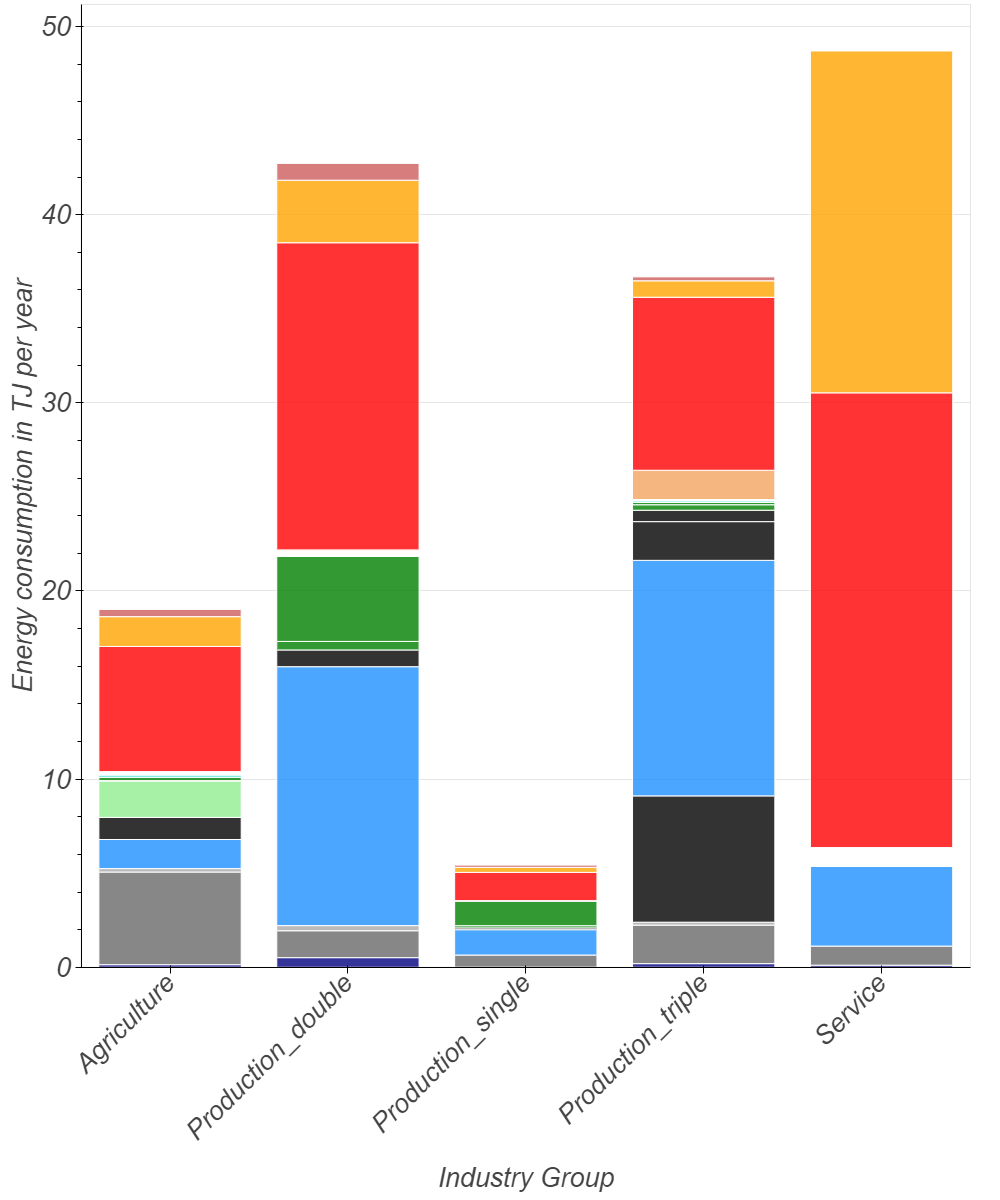
\includegraphics[width=\linewidth]{Img/dan_ind/overview_total.png}
\end{minipage}%
\begin{minipage}{.3\textwidth}
  \centering
  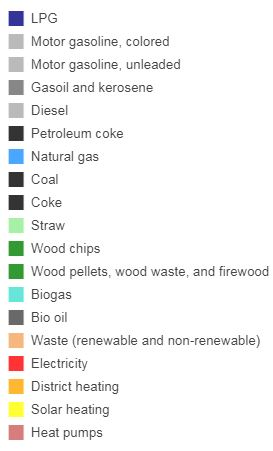
\includegraphics[width=\linewidth]{Img/dan_ind/legend}
\end{minipage}
  \caption{Total energy use in Danish industry groups by fuel \cite{VM2015}}
  \label{total_use} 
\end{figure}


COMMENTS FOR THE FIGURE:
\begin{itemize}
    \item Remove transport from fuels (transport and transport machinery) CHECK
    \item Maybe report the percentages?
    \item One image with bars and legend
\end{itemize}

It´s relevant to notice that the fuel consumption among the sectors is distributed un-evenly, with electricity (36\%), natural gas (21\%), district heating (15\%), gasoil/kerosene (6.4\%) and petroleum coke (4\%) covering the majority of the consumption, while the other fuels contribute partially.

\autoref{heatmapagri}, \autoref{heatmapprod}, \autoref{heatmapserv} provide an indication on the fuel-use for the different industrial processes. 

\begin{figure}[H]
\centering
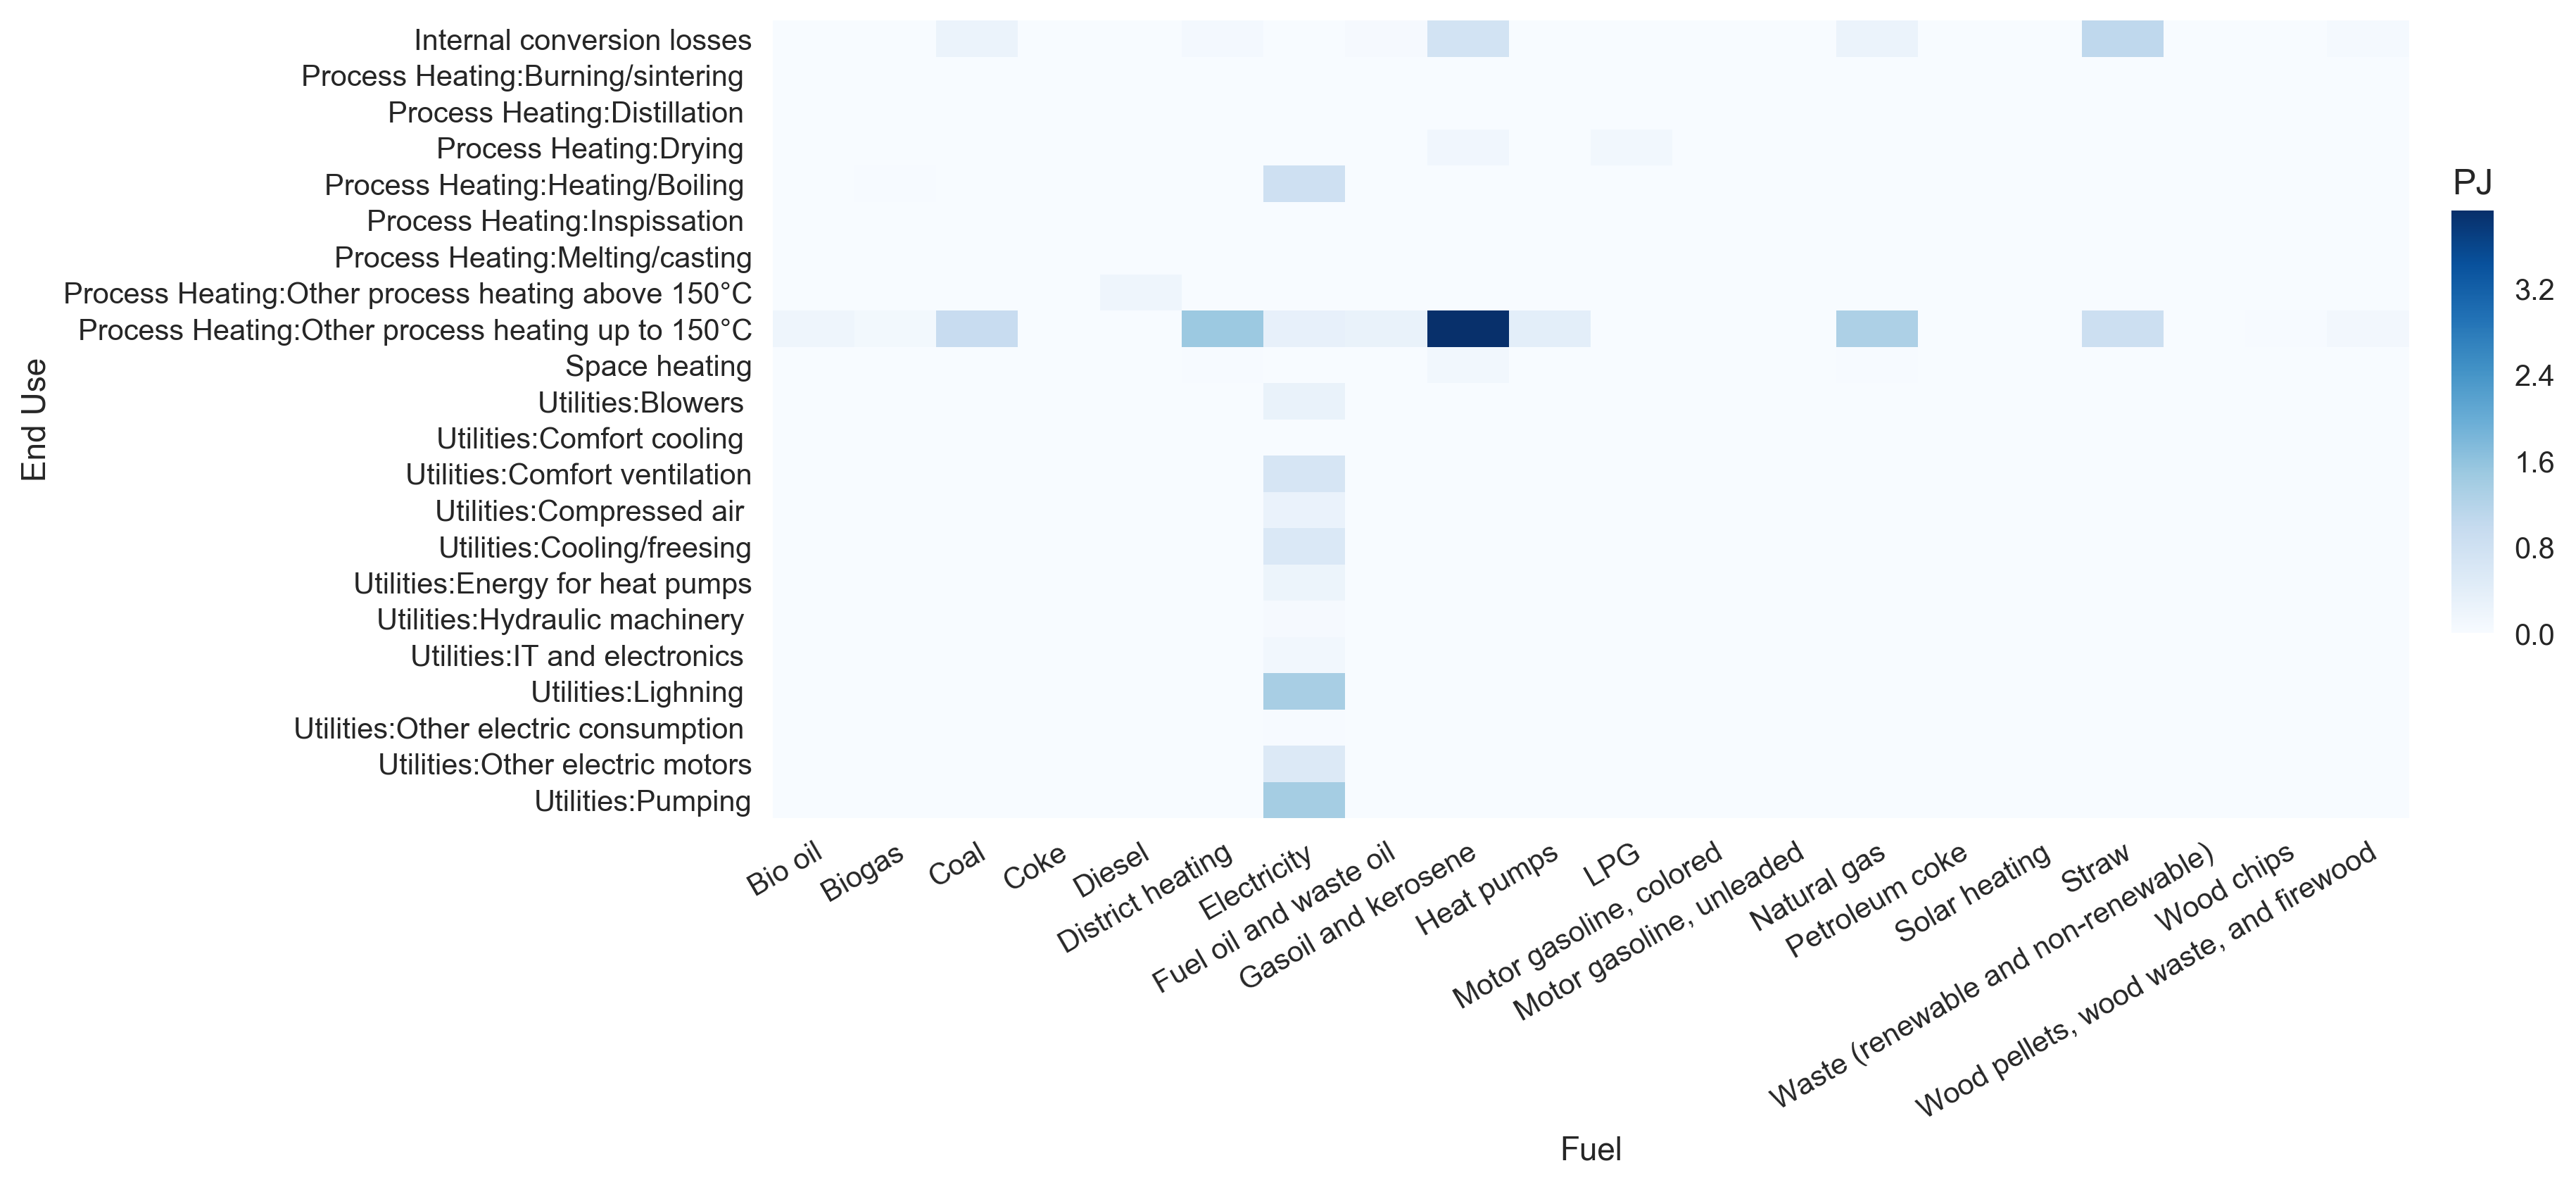
\includegraphics[width=\linewidth]{Img/dan_ind/heatmap_agri.png}
\caption{Breakdown of energy consumption by end-use and fuel in agriculture\cite{VM2015}}
\label{heatmapagri} 
\end{figure}

\begin{figure}[H]
\centering
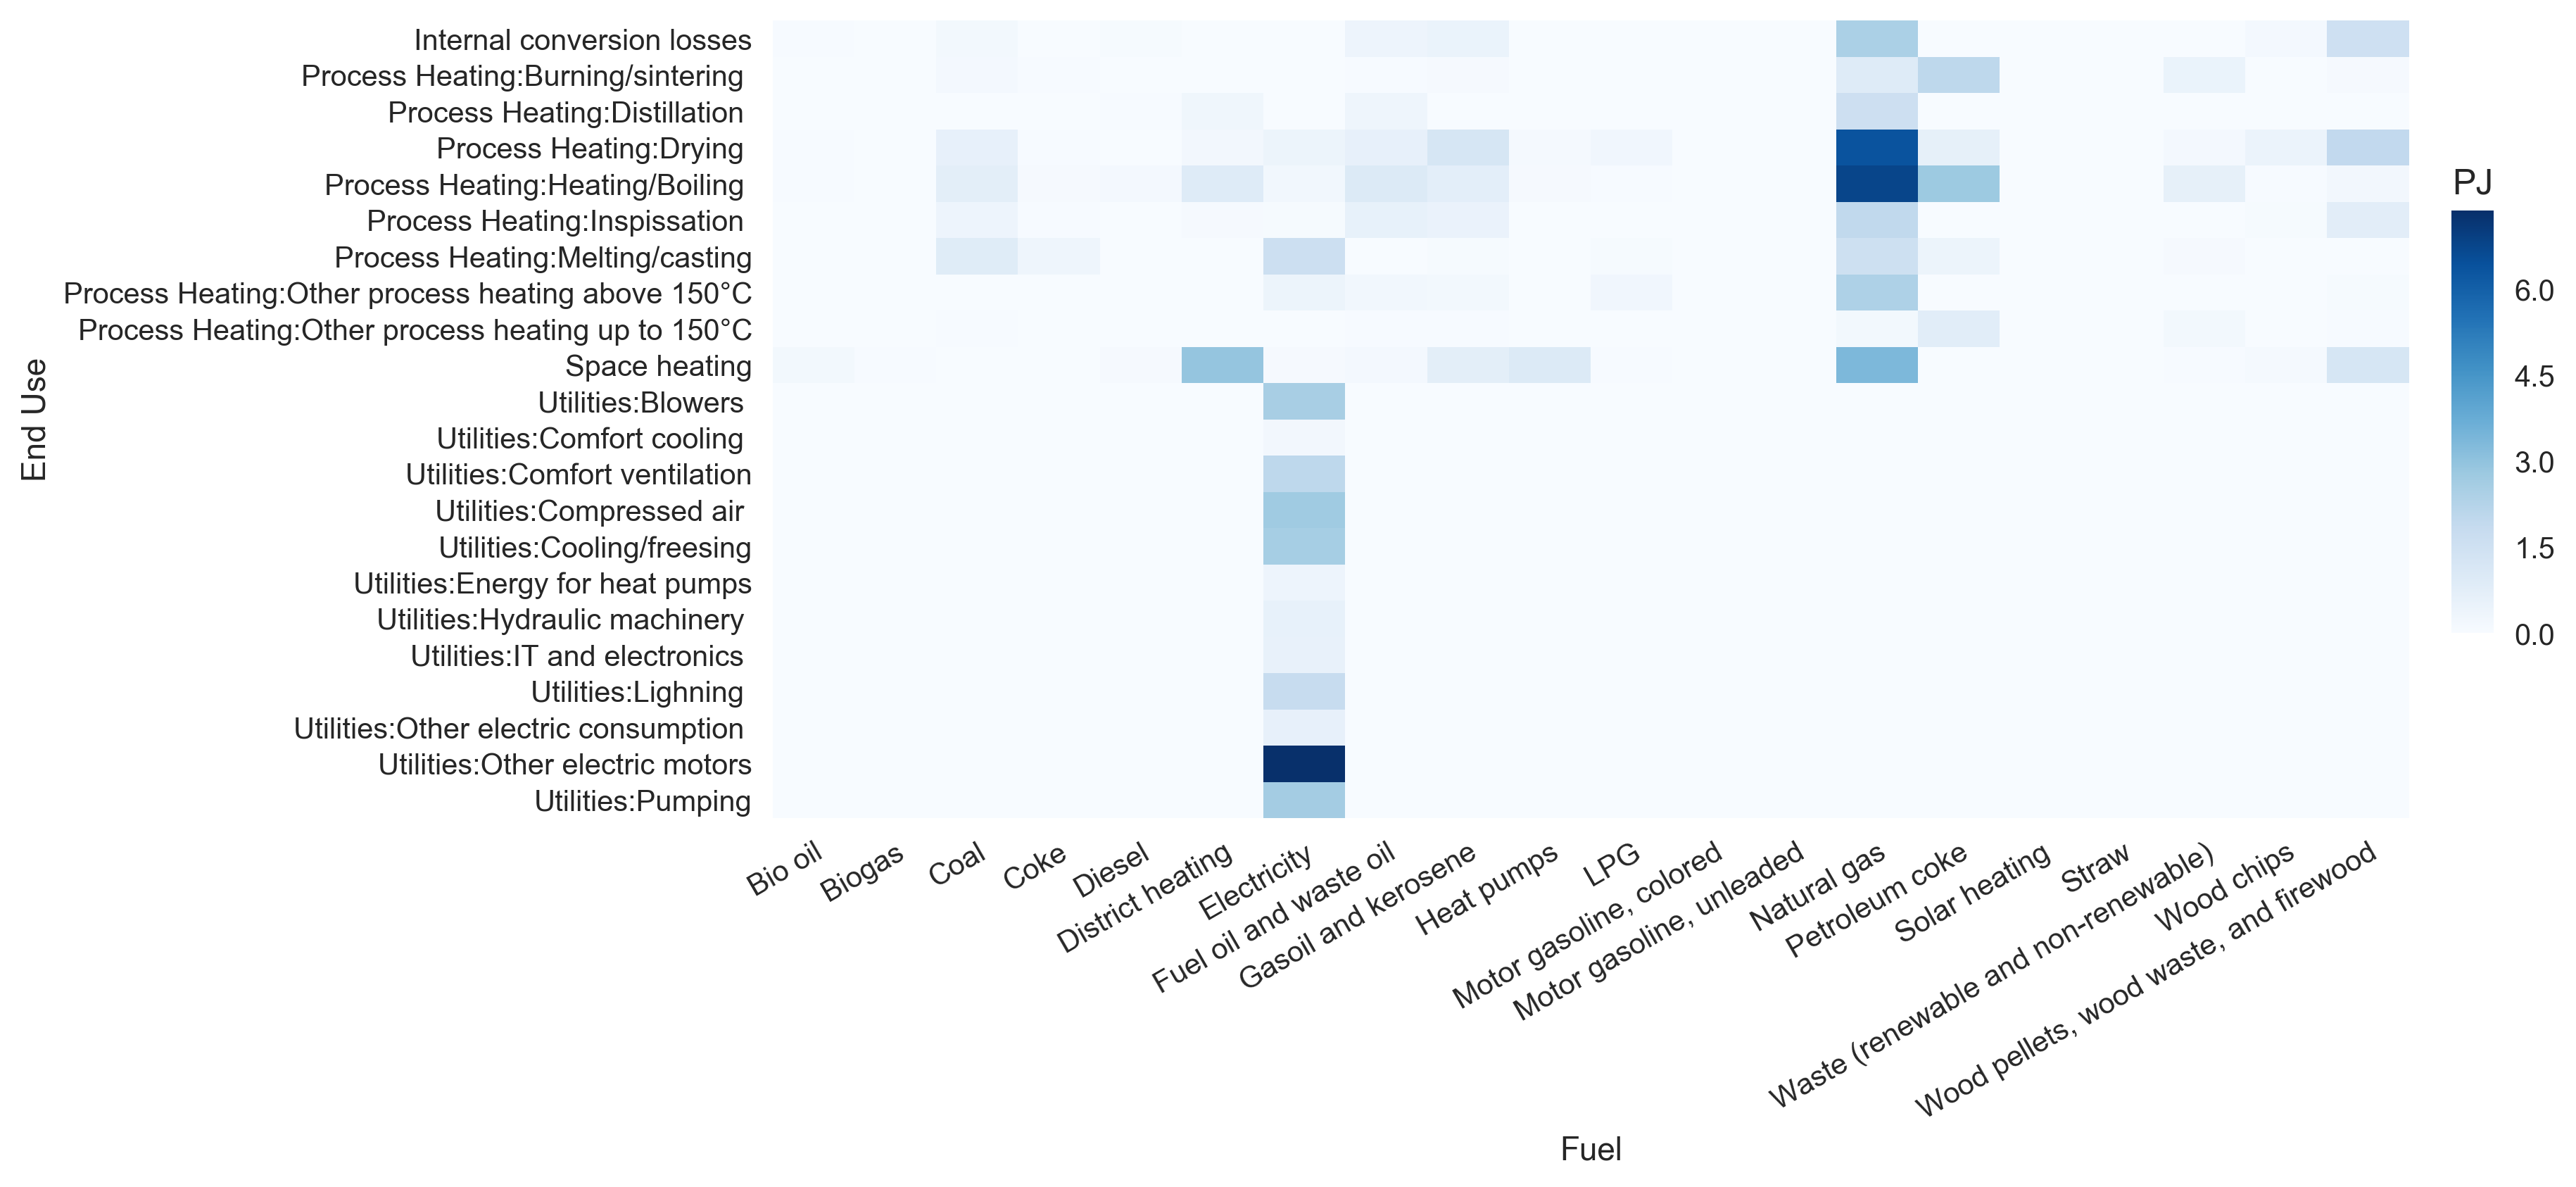
\includegraphics[width=\linewidth]{Img/dan_ind/heatmap_prod.png}
\caption{Breakdown of energy consumption by end-use and fuel in production\cite{VM2015}}
\label{heatmapprod} 
\end{figure}

\begin{figure}[H]
\centering
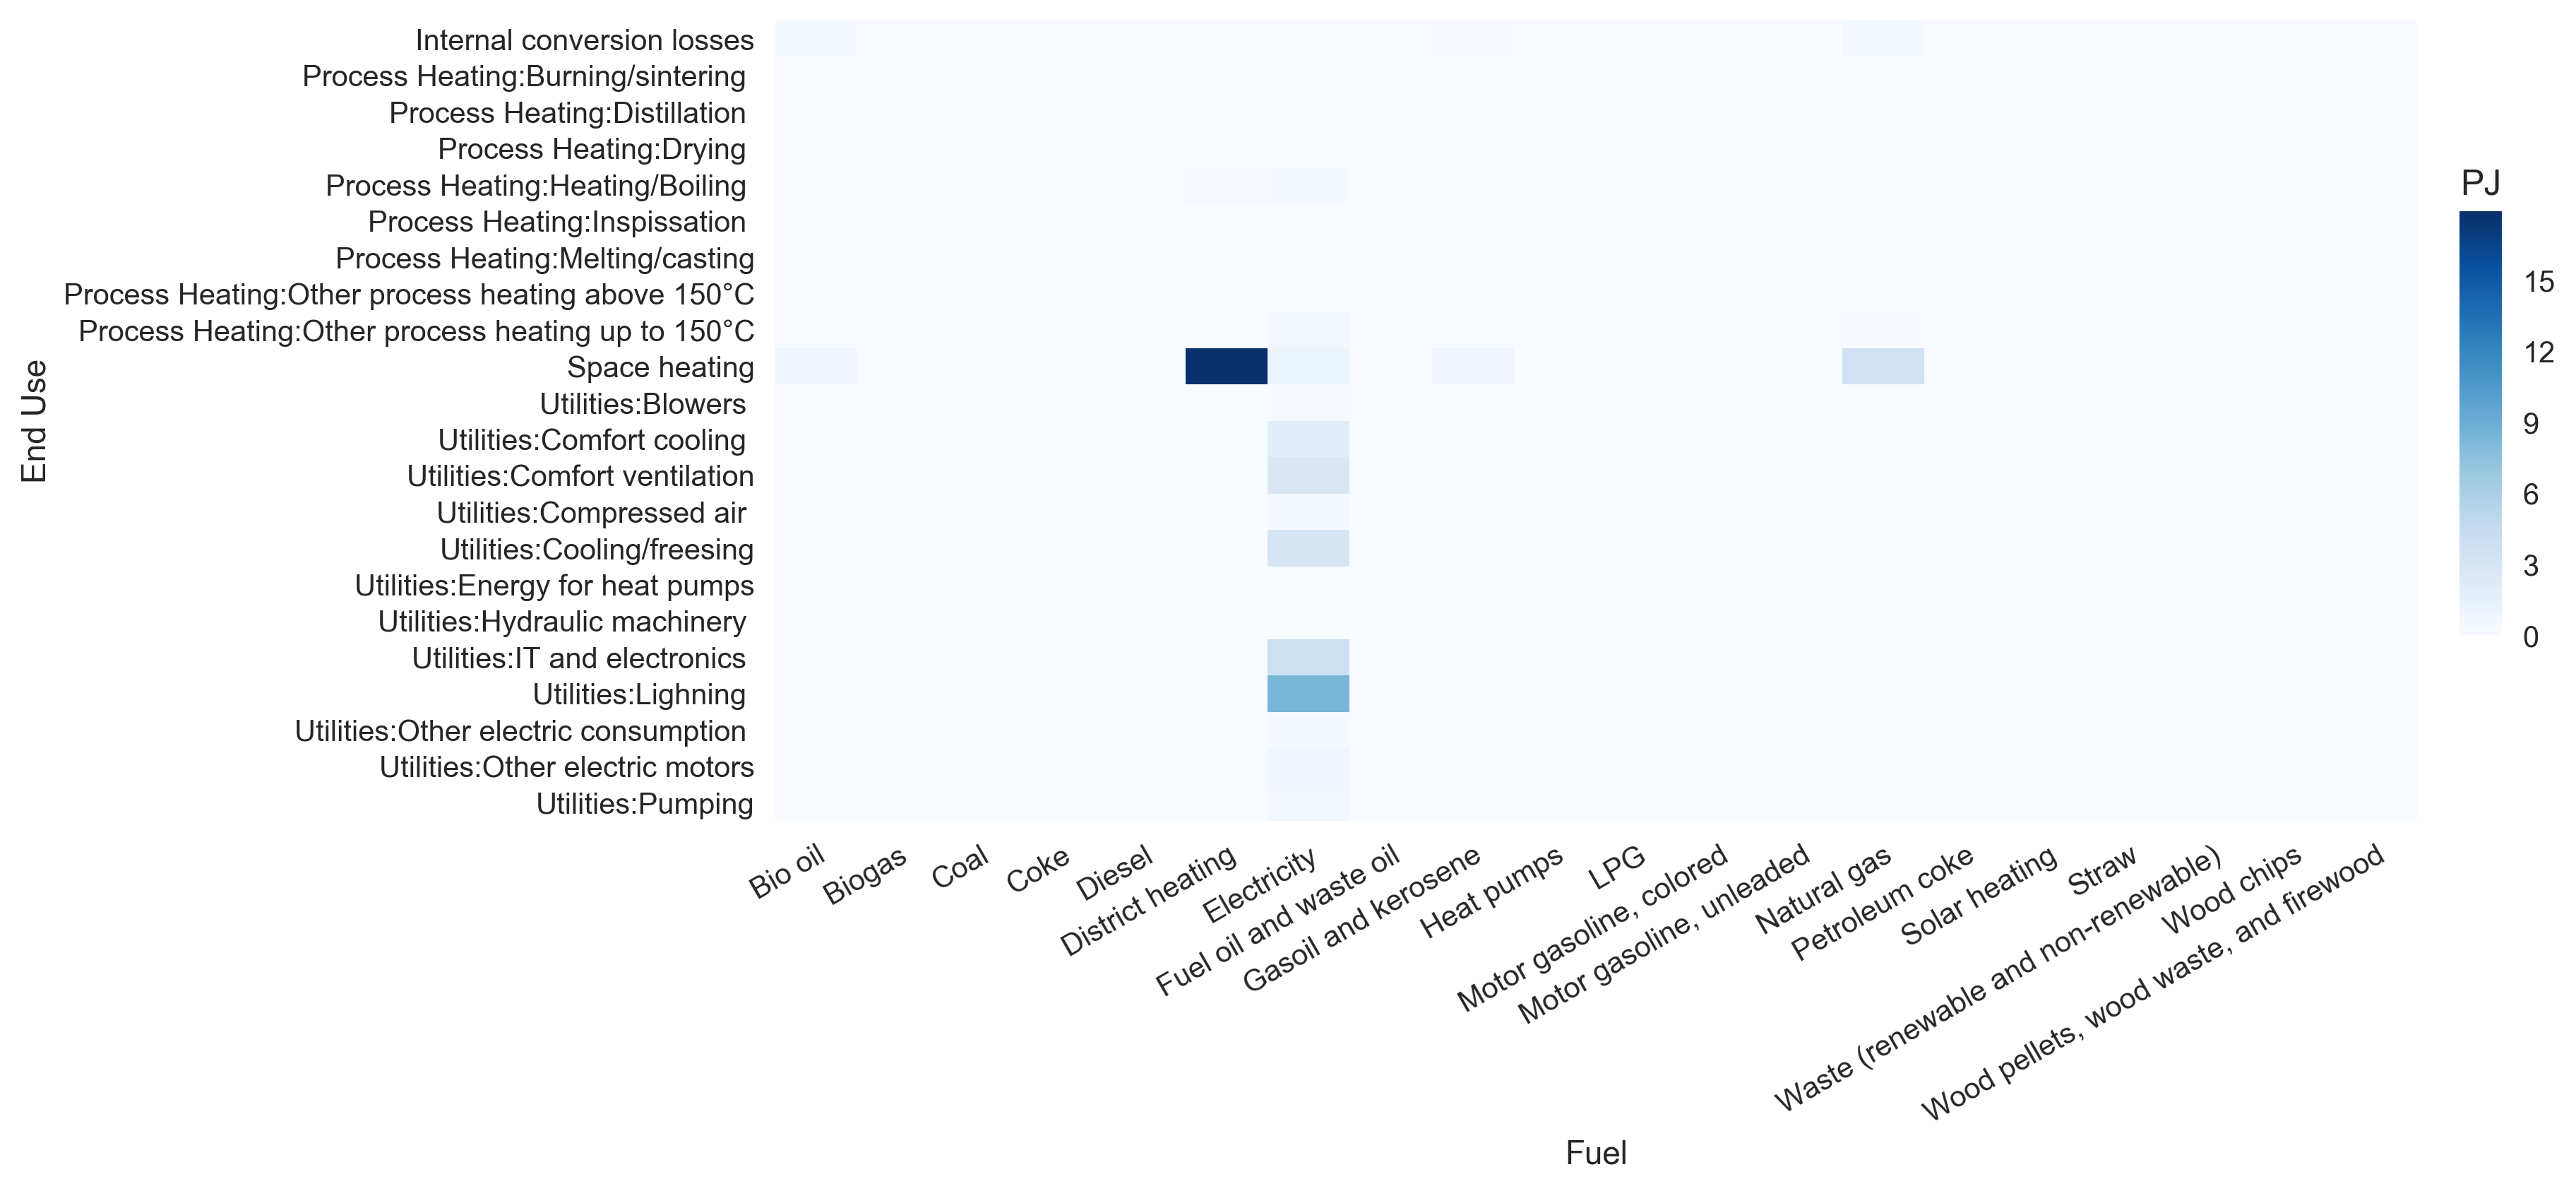
\includegraphics[width=\linewidth]{Img/dan_ind/heatmap_serv.png}
\caption{Breakdown of energy consumption by end-use and fuel in services\cite{VM2015}}
\label{heatmapserv} 
\end{figure}

The heat maps, presented in three clustered groups, provide a useful indication on the most energy-intensive processes and on the most employed fuels. 
In agriculture, most of the fuel consumption is related to heating up to 150\textdegree (51\%); in production, drying (15\%), heating/boiling (16\%) and space heating (11\%) are predominant; while in service, space heating (50\%) and lightning (17\%) together consumer more than half of the total fuels used.

In production, there is a high diversity of end-use while the role of gas as a fule is predominant. 
Space heating and transport dominate the total energy use in the service sector. While most space heat already supplied by district heat, natural gas is the second.

Furthermore, the data show an un-even distribution of fuel consumption in the various groups, with electricity (34\%) and gasoil/kerosene (25\%) being predominant in agriculture, electricity (31\%) and natural gas (31\%) in production, and electricity (50\%) and district heating (37\%) dominating the service sector.

\\
This preliminary description of the Danish industry poses the bases for the modelling of the sector and the investigation of decarbonisation options. Indeed, with a clear overview of the end-use processes and the related fuel consumption, the industry sector can be conveniently integrated in an energy system model. 
The following section proposes a mathematical model for the industry sector and investigates on extensions to analyse decarbonisation options. 



%%%%%%%%%%%%%%%%%%%%%%%%%%%%%%%%%%%%%%%%%%%%%%%%%%%%%%%%%%%%%%%%%%%%%%%%%%%%%%%%%%%%%

\section{Methodology} \label{meths}

%%%%%%%%%%%%%%%%%%%%%%%%%%%%%%%%%%%%%%%%%%%%%%
\subsection{Balmorel, an energy system model}

The use of energy system models is useful to assess the role of industry in achieving pathways to decarbonised energy systems. As commodities like electricity and heat are highly related, in both power and industry sector (e.g. due to the use of heat pumps), only a simultaneous consideration can reflect the cost-minimal solutions from a system perspective. This allows to investigate what is usually defined as "socio-economic welfare maximisation" under different conditions. 
Among the tools available in the literature \cite{Connolly2010}, the energy system model Balmorel is adopted for the analysis \cite{balmorel}.
Balmorel is an energy system, linear programming, open source model that optimises investments and operation of power plants, storage devices and transmission lines in an international perspective \cite{Ravn2001}. 
The model considers a set of neighbouring countries operating in an interconnected electricity market. Each country is composed by one or several regions. Electricity can be traded and transmitted between adjacent regions, with limits imposed by given transmission capacity. 
To consider the heat sector, each electricity region is divided into several district heating areas. Heat transmission among such areas is not allowed.  
\\
Balmorel considers time according to years, seasons (weeks) and individual time units (hours). 
The user can freely decide the time horizon of the analysis and the choice depends on the needs for the specific investigation. 
\\
The model allows to simulate scenarios where demand and supply of electricity and heat are balanced with operations and investments, considering local generation vs. import/export, price elasticity of the demand and other characteristics typical of the energy systems \cite{Munster2012}. 
\\
The model relies on a set of exogenous input data, including capacities of electricity and heat generation technologies, transmissions lines and heat and power demand. 
Energy generating technologies include CHP (both back-pressure and extraction), heat pumps, storage devices (for electricity and heat), and renewable based production technologies (hydro, wind, solar).
Additional key assumptions relate to fuel prices, CO2 costs, taxes and support schemes are required for specific analysis.
The original data available in the model can be modified for personal application in specific analyses. This allows Balmorel to be adapted for specific investigations that are not presently covered by the standard version of the model \cite{Wiese}.
\\
The model has been previously applied for a wide range of studies, such as integration of renewable technologies in the energy mix, analysis of market conditions, policies implementation, future role of district heating and impact of energy efficiency technologies in the energy system \cite{Ball2007,Jensen2008,Karlsson2008,Munster2012,Munster2010,Baldini2016a}.
In the next section, we will propose a modelling representation of the industry sector, as the Balmorel model lacks a comprehensive representation of the industry. Enhancing the model with details about industrial energy use and processes will improve the quality of the analyses and provide more details on the impact, in the energy system, of changes in the industrial sector.

%%%%%%%%%%%%%%%%%%%%%%%%%%%%%%%%%%%%%%%%%%%%%%
\subsection{Modelling of the industrial sector}

%%%%%%%%%%%%%%%%%%%%%%%%%%%%%%%%%%%%%%%%%%%%%%
\subsection{Modelling of decarbonisation options}

\paragraph{Electrification}

\paragraph{Fuel substitution}

\paragraph{Excess heat}

\paragraph{Energy savings}


%Provide sufficient details to allow the work to be reproduced by an independent researcher. Methods that are already published should be summarized, and indicated by a reference. If quoting directly from a previously published method, use quotation marks and also cite the source. Any modifications to existing methods should also be described.
Industry plays a decisive part in the integrated energy system. The following energy system analysis questions appear:
\begin{itemize}
    \item Saving potential
    \item Fuel shift potential to gas, renewable gas
    \item Electrification potential
    \item Flexibility potential
    \item Usage of excess heat
    \item Usage of district heating
\end{itemize}
For an integrated modelling approach, a high level of detail required for
\begin{itemize}
    \item Fuel Usage
    \item End-use: electricity, heat specified by temperature levels
    \item Time: Temporal demand profiles
    \item Geography: Vicinity to heat demand / district heat network
    \item Industry group
\end{itemize} 
% \begin{itemize}
%     \item Overview whole model (Balmorel)
%     \item Zoom into industry add on (Figure)
%     \item Describe concept behind industry add on and heat transfer including formulas
%     \item Level of detail: Geographically, technologies, end-use
%     \item Data derivation (Could also be an own section or subsection)
% \end{itemize}

%%%%%%%%%%%%%%%%%%%%%%%%%%%%%%%%%%%%%%%%%%%%%%%%%%%%%%%%%%%%%%%%%%%%%%%%%%%%%%%%%%%%%

\section{Case study / empirical data} \label{datadescr}

%%%%%%%%%%%%%%%%%%%%%%%%%%%%%%%%%%%%%%%%%%%%%%

In this paper, Denmark is taken as a case study for modelling the transition to carbon neutrality in the industrial sector. On one hand Denmark covers a wide range of different industries but  and on the other hand the amount of industrial processes still possible to handle to get an impression of the effects of modelling it more in detail in the integrated energy system. Furthermore data availability in Denmark is extensive compared to other countries. This makes it an suitable focus area, in which data processing and modelling methods can be tested with real data, that is still manageable. However, methods can be principally applied to other areas.

\subsection{Overview Data Sources and Processing}
The Danish case study is based on the following main datasets:
\begin{itemize}
 \item Yearly Danish energy usage by industrial group (db117-grouping) and fuel type (..different fuels)
 \item End-use connected to fuel type and industry groupings for a specific year (2012) 
 \item Danish companies including address, industry group and number of employees
 \item Adress database connecting the address to geographic location
 \item Geographic location and extension of district heat areas
 \item Conversion potential for electrification and biomass in shares per industry grouping
 \item Hourly gas consumption profiles of gas consumers including the information of the industry group affiliation
\end{itemize}

As far as possible, openly available data was chosen for the case study. Like that results can be scrutinized based on the open soucre code and open sources. However, consumer profiles can only be published in aggregated form.

For data processing, the python packages pandas and numpy were utilized, which dataframe structure is especially suited for processing and combination of different data source wiht a satisfactory speed performance. With the objective of achieving a high re-usability and flexibility of data and scripts, the processing was modularized and split in different steps. Between the scripts, intermediate dataframes are passed. This makes the processing more efficient, since some dataframes have to be applied by different subsequent steps. This flow is illustrated in Figure ...  

%%%%%%%%%%%%%%%%%%%%%%%%%%%%%%%%%%%%%%%%%%%%%%

\subsection{Energy use}
The energy consumption by industry group and fuel type is published by Statistics Denmark on a yearly basis. This data is reliably and continously available and the structure of the industry grouping follows the db117-code which is widely applied for identifying the affiliation of companies and utilized in other data sources about the conversion potential in industry. From that dataset, public service, building and mining was excluded.

On the end-use side, transport of all industry groups is excluded from the dataset and the case study focuses on electricity and heat demand. The required temperature level is decisive for which conversion options are available to reduce the use of fossil fuels. The allocation of the fuel usage in industry to different end-use categories is available for the year 2012 from the ... for a large part of Danish industry. The absolute fuel consumption numbers per end-use, fuel and industry group were converted to shares relating to industry groups and fuel usage. Due to the fact that the industry groups were choses slightly different than in Statistics Danmarks, this had to be accounted for. Also, fuels and industry grouping had to be aligned. This calculation can be applied to each available year of the Statistics Denmark data, so that after this calculation step the energy usage per industry group, fuel and end-use is available for different years. It has to be mentioned that the division has to be adapted if the end-use within an industry group changes significantly. Growth of industry groups and thus energy usage increase would be divided by the same end-use allocation.

Derived from the conceptual model, we group the end-use heat demand into space heat, process heat low and process heat high. This was considered detailed enough to caputure the main differences between the conversion option while still modelwise manageable. ...end-use heat categories were available from the main data, which are - depending on their required temperature level aggregated as displayed in Table ...

\begin{table}
\begin{tabular}{l | c | c}
End-use & Temperature level [$^{\circ}$C] & Model heat type\\
\hline \hline
Space heating & 50-90 & space  \\ 
Distillation & 50-100 & process low \\
Heating/Boiling & mostly 70-110 & process low \\
Drying & about 100 & process low \\
Inspissation & 130 & process low \\ 
Burning/Sintering & more than 250 & process high \\ 
Melting/Casting & more than 300 & process high  
\end{tabular}
\caption{Clustering end-use by heat level. Source for process heat levels: \cite{VM2015}}
\end{table}

%%%%%%%%%%%%%%%%%%%%%%%%%%%%%%%%%%%%%%%%%%%%%%

\subsection{Profiles}
\subsubsection{Demand profiles: Electricity}

The following figures show the variability of the resulting electricity profiles. To illustrate the main patterns, the frequency distribution of the relative consumption values over the whole year is given as boxplots aggregated by the main industry groups (\ref{fig:boxplots}). Seasonal variation of the electricity demand differing by industry group is shown in Figure \ref{fig:trendlines}.

\begin{figure}[H]
\centering
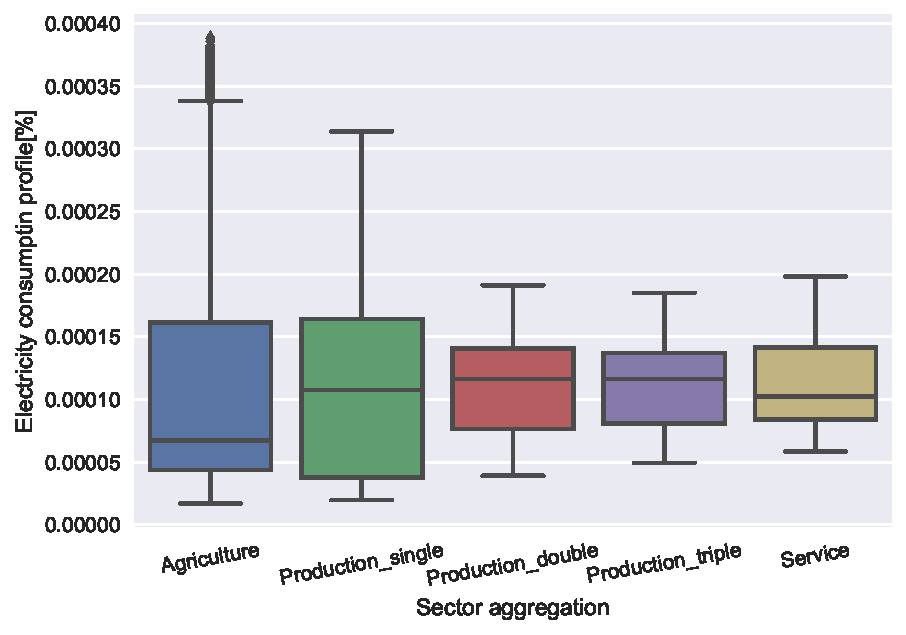
\includegraphics[width=\linewidth]{Img/profiles/boxplots.pdf}
\caption{Boxplots of relative electricity consumption. Own calculations based on \cite{Energinet.dk,NordPool2016,ElforbrugsPanelerne2015,Andersen2013a,Andersen2013b,VM2015}}
\label{fig:boxplots} 
\end{figure}

\begin{figure}[H]
\centering
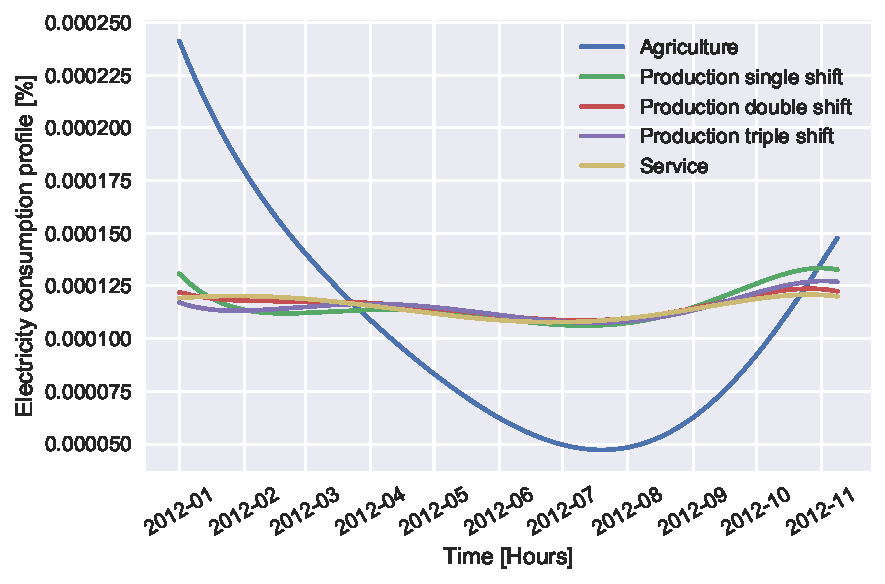
\includegraphics[width=\linewidth]{Img/profiles/trendlines.pdf}
\caption{Relative variation of seasonal electricity consumption, trend-lines (fit to the 18th order). Own calculations based on \cite{Energinet.dk,NordPool2016,ElforbrugsPanelerne2015,Andersen2013a,Andersen2013b,VM2015}}
\label{fig:trendlines}
\end{figure}

\subsubsection{Demand profiles: Space heat}
Figure \ref{fig:heat_space_year} and \ref{fig:heat_space_week} show the derived profiles of space heating. There is a clear indication of the seasonal and the weekly variation.

\begin{figure}[H]
\centering
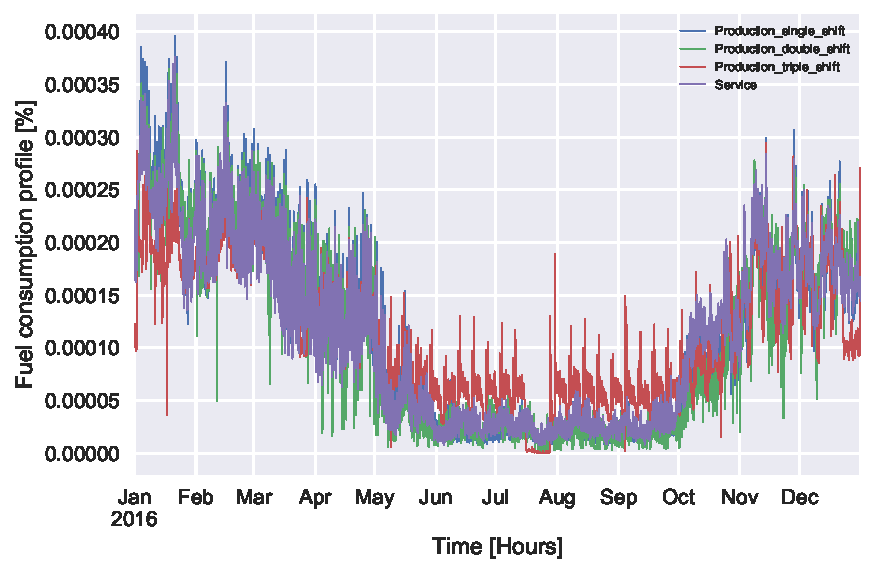
\includegraphics[width=\linewidth]{Img/profiles/heatprofile_space_year_perc.pdf}
\caption{Yearly scale. Own calculations based on data from \cite{DanskGasDistribution2016,VM2015}}
\label{fig:heat_space_year}
\end{figure}
	
\begin{figure}[H]
\centering
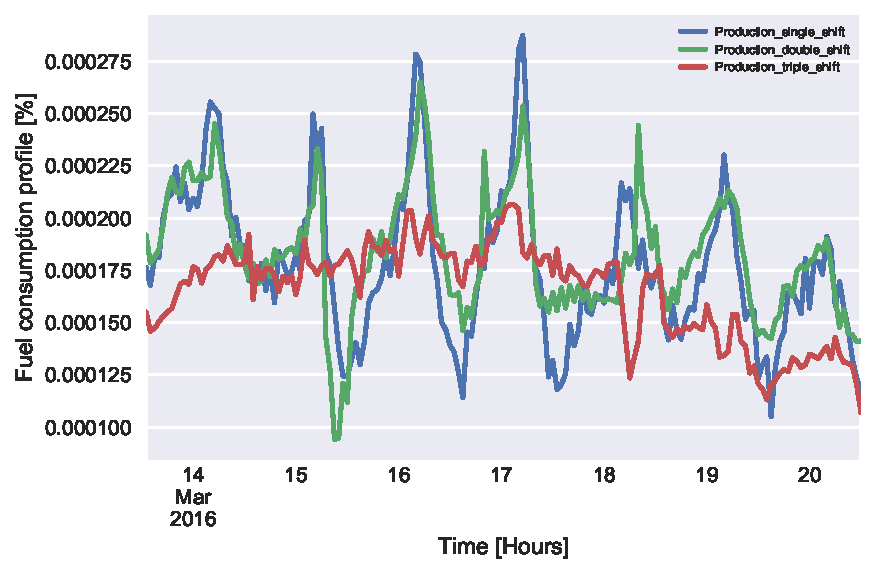
\includegraphics[width=\linewidth]{Img/profiles/heatprofile_space_week_perc_noserv.pdf}
\caption{Sample week. Own calculations based on data from \cite{DanskGasDistribution2016,VM2015}}
\label{fig:heat_space_week}
\end{figure}

\subsubsection{Demand profiles: Process heat}
For process heating the variation due to work hours according to holidays (Figure \ref{fig:heat_process_year} and due to the weekly routine (Figure \ref{fig:heat_process_week} is clearly distinguishable.

\begin{figure}[H]
\centering
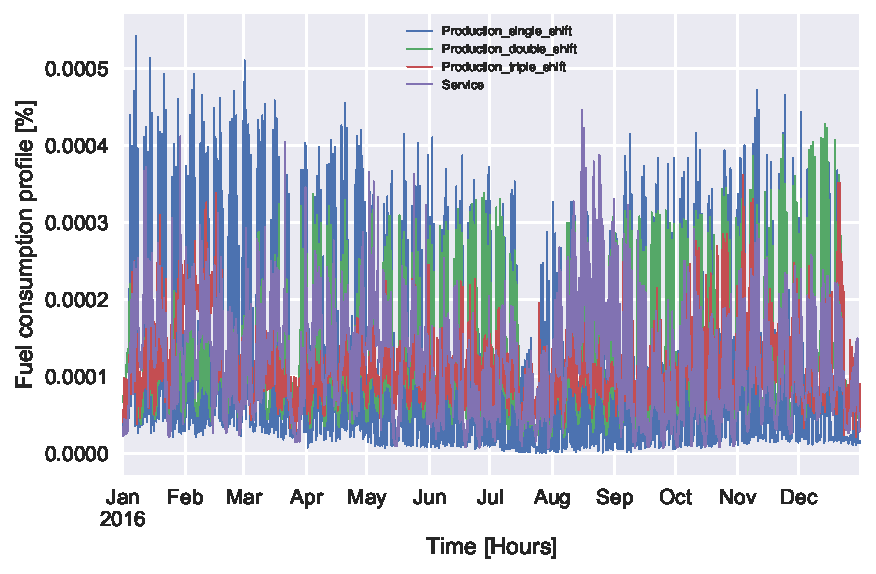
\includegraphics[width=\linewidth]{Img/profiles/heatprofile_process_year_perc.pdf}\\
\caption{Yearly scale. Own calculations based on data from \cite{DanskGasDistribution2016,VM2015}}
\label{fig:heat_process_year}
\end{figure}
	
\begin{figure}[H]
\centering
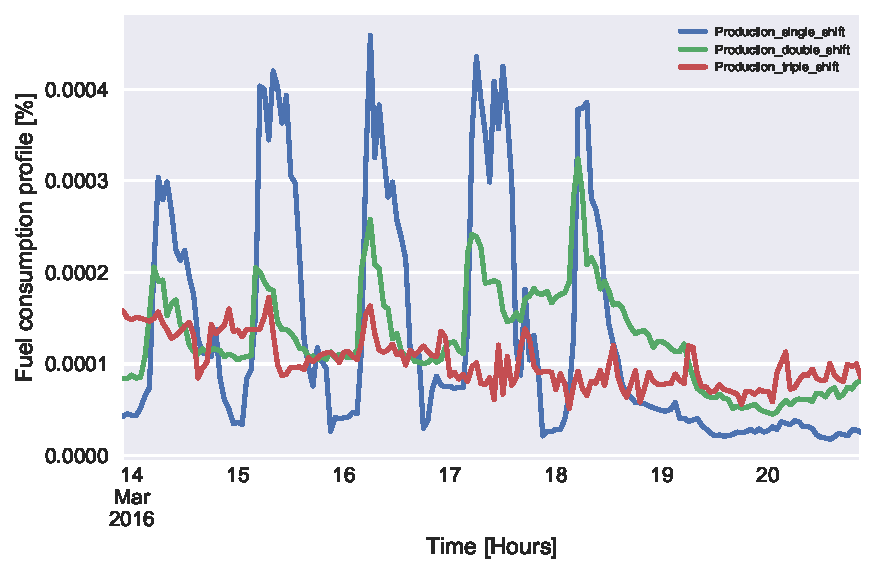
\includegraphics[width=\linewidth]{Img/profiles/heatprofile_process_week_perc_noserv.pdf}\\
\caption{Sample week. Own calculations based on data from \cite{DanskGasDistribution2016,VM2015}}
\label{fig:heat_process_week}
\end{figure}

%%%%%%%%%%%%%%%%%%%%%%%%%%%%%%%%%%%%%%%%%%%%%%

\subsection{Geographical mapping of industrial energy consumption}
District heating plays a major role in Denmark. ... \% of of space heat demand is supplied via ... district heat networks. Provided that the supply of the district will be transformed to completely renewable ones (source), an increased use of district heat for space and process heat for industry is an important option to reduce fossil fuel usage. The feasibility of this option depends on the location of this industrial demand. Whether the company is within or close to a district heating area decides whether this option can be used. Depending on the required temperature, heat pumps would be necessary to raise the provided temperature. The vicinity to such a network is furthermore decisive for the possibility of excess heat usage. Connection to a district heat network offers the possibility to exploit the otherwise lost heat potential beyond recycling it on site.

The basis this localalisation is the list of companies located in Denmark which includes addresses, affiliation to detailed industry group and number of employees information \cite{virk2017}. Entries that did not have any employees reduced the list from .... to .... The geographic location (coordinates) for the remaining were derived by matching the addresses to an address list containing coordinates \cite{}. This was done via a matching operation in python.

The method for localisation of the industry demand is based on the employee shares of industrial groups of companies.

\textit{from addresses, companies - location - to DH areas (could also be done for gas areas), how many not localized, which ones taken out - employee share per group approach - verification}

%%%%%%%%%%%%%%%%%%%%%%%%%%%%%%%%%%%%%%%%%%%%%%

\subsection{Decarbonisation option potentials}
\textit{maybe a table with the different options and if they are applicable for process heat high, low and space heat and make an indication if they are rather expensive or rather cheap / subsection could also be before geographical subsection}


%%%%%%%%%%%%%%%%%%%%%%%%%%%%%%%%%%%%%%%%%%%%%%%%%%%%%%%%%%%%%%%%%%%%%%%%%%%%%%%%%%%%%

\section{Preliminary outcomes and discussion} \label{outcdisc}
% Results should be clear and concise.
Concluding the numbers. This I know how to calculate:
\begin{itemize}
    \item How much industry already uses district heat?
    \item How much industry already uses heat pumps?
    \item How high is the potential for more industry using district heat?
    \item Which percentage/amount of fossil fuel/installed capacity can be electrified to which cost in which industry group (DGC-data)?
    \item What is the fuel switch options to which cost: Maybe we should have a table with the sectors and end-uses their options to decarbonize.
\end{itemize}
This would be nice to get, but probably only modelling possible:
\begin{itemize}
    \item electricity, process, space heat saved
    \item process, space heat electrified
    \item fuel switched
    \item district heating utilized by industry
    \item excess heat utilized additionally from industry
    \item costs
    \item emissions saved
    \item sensitivities
\end{itemize}

%DISCUSSION
% This should explore the significance of the results of the work, not repeat them. A combined Results and Discussion section is often appropriate. Avoid extensive citations and discussion of published literature.
\begin{itemize}
    \item discuss the derived numbers: upper or lower bound, how good can they be? Where do we need to go further?
    \item Which options to decarbonize industry are promising from that numbers? Where do we need to go deeper?
    \item What would be different in other countries? More heavy industry etc.
    \item main other barriers for introducing these that are difficult to capture
    \item policy implications?
    \item further research needs
\end{itemize}

\subsection{Future work}

%%%%%%%%%%%%%%%%%%%%%%%%%%%%%%%%%%%%%%%%%%%%%%%%%%%%%%%%%%%%%%%%%%%%%%%%%%%%%%%%%%%%%

\section{Conclusion} \label{endofpaper}
% The main conclusions of the study may be presented in a short Conclusions section, which may stand alone or form a subsection of a Discussion or Results and Discussion section.

%%%%%%%%%%%%%%%%%%%%%%%%%%%%%%%%%%%%%%%%%%%%%%



%%%%%%%%%%%%%%%%%%%%%%%%%%%%%%%%%%%%%%%%%%%%%%%%%%%%%%%%%%%%%%%%%%%%%%%%%%%%%%%%%%%%%

\section*{Acknowledgements}
The research has been co-financed by Innovation Fund Denmark under the research project SAVE-E, grant no. 4106-00009B and by XXX under the research project FUTURE GAS, grant no. .
The authors also thank the institutions which gave access to relevant data: the Danish Energy Agency (Energistyrelsen, DEA) and the energy consulting company Viegand Maagøe.
This paper develops on work presented first at the $12^{th}$ SDEWES 17 Conference on sustainable development of energy, water and environment systems at Dubrovnik, Croatia.
%Collate acknowledgements in a separate section at the end of the article before the references and do not, therefore, include them on the title page, as a footnote to the title or otherwise. List here those individuals who provided help during the research (e.g., providing language help, writing assistance or proof reading the article, etc.).

% Formatting of funding sources
%List funding sources in this standard way to facilitate compliance to funder's requirements:

%Funding: This work was supported by the National Institutes of Health [grant numbers xxxx, yyyy]; the Bill & Melinda Gates Foundation, Seattle, WA [grant number zzzz]; and the United States Institutes of Peace [grant number aaaa].

%It is not necessary to include detailed descriptions on the program or type of grants and awards. When funding is from a block grant or other resources available to a university, college, or other research institution, submit the name of the institute or organization that provided the funding.

%If no funding has been provided for the research, please include the following sentence:

%This research did not receive any specific grant from funding agencies in the public, commercial, or not-for-profit sectors.

%%%%%%%%%%%%%%%%%%%%%%%%%%%%%%%%%%%%%%%%%%%%%%%%%%%%%%%%%%%%%%%%%%%%%%%%%%%%%%%%%%%%%

\section*{Comments for final check}

\begin{itemize}
    \item all needs to be decarbonized, but industry especially difficult and diverse
    \item define industry for our paper
    \item Non-residential energy demand (industry) constitutes a
substantial share of total energy demand
    \begin{itemize}
        \item EU: production and agriculture 28\% / services 13\% \cite{Eurostat2017}
        \item Denmark: production and agriculture 20\% / services 13\% \cite{DanishEnergyAgency2014}
    \end{itemize}
    \item Usage of energy in industry is diverse regarding
        \begin{itemize}
            \item End-use / required type of energy / temperature levels
            \item Fuels
            \item Temporal profiles
            \item Demand flexibility
        \end{itemize}
    \item Solutions and challenges to go 100\% renewable are diverse
    \item Interaction with the rest of the energy system decisive
    \item Thus, it is important to model in detail and in the context of the whole integrated energy system
    \item review on what has been done for industry modelling (method-wise) and what came out (numbers)
    \item explain scope and focus on Denmark?
    \item outline paper: This paper gives 
\end{itemize}




%%%%%%%%%%%%%%%%%%%%%%%%%%%%%%%%%%%%%%%%%%%%%%%%%%%%%%%%%%%%%%%%%%%%%%%%%%%%%%%%%%%%%


%%%%%%%%%%%%%%%%%%%%%%%%%%%%%%%%%%%%%%%%%%%%%%%%%%%%%%%%%%%%%%%%%%%%%%%%%%%%%%%%%%%%%

\section*{References}

\bibliography{mybibfile}

%%%%%%%%%%%%%%%%%%%%%%%%%%%%%%%%%%%%%%%%%%%%%%%%%%%%%%%%%%%%%%%%%%%%%%%%%%%%%%%%%%%%%


\end{document}